\documentclass{article}
\usepackage[a4paper, bindingoffset=0 cm, left=2.5cm, right=2.5cm, top=1.5cm, bottom=1.5cm, footskip=0.5cm]{geometry}
\usepackage[utf8]{inputenc}
\usepackage[english]{babel}
\usepackage{mdframed}
\usepackage{tikz}
\usepackage{biblatex}
\usepackage{csquotes}
\addbibresource{literature.bib}
\usepackage{hyperref}
% Added for the figures and tables of this paper
\usetikzlibrary{positioning,arrows.meta}
\usepackage{graphicx}
\usepackage{booktabs}
\usepackage{amsmath}
\usepackage{amssymb}
\usepackage{caption}
\usepackage{subcaption}
\captionsetup{font=small}

\title{1JM0211 Process Mining \\Mining Organizational Patterns}
\author{Group 5, Members: Sophie Veltmans, Lotte van der Vlies, Gijs Kruize}
\date{Submission Date}

\begin{document}
\newmdenv[linewidth=1.5pt, frametitlerule=true, roundcorner=3pt]{mybox}
\pagestyle{empty}
\let\svmaketitle\maketitle
\def\maketitle{\svmaketitle\thispagestyle{empty}}
\maketitle

\begin{mybox}[frametitle = Remarks (to be removed upon submission)]
Page limit: 5 pages excluding references; use appropriate scientific references where possible \cite{DBLP:books/sp/Aalst16}; your short paper shall follow the structure outlined below
\end{mybox}


\section{Motivation and Scientific Background}\label{sec:motivation}
Organizational mining studies who performs which activities, which resources
play similar roles and how work is handed over~\cite{song2008organizational,
vanderaalst2005social}. Classical results such as handover-of-work networks
describe relations between actors, but not \emph{which tasks} they perform
together and in which structure. Discovering a process model on
activity--resource labels does show this, but with many resources it yields
unreadable ``spaghetti'' models. Diamantini et al.~\cite{diamantini2016behavioral}
therefore build one \emph{instance graph} per case, which shows the order and
the parallelism of its events, and mine the most relevant subgraphs over all
instance graphs. Such a \emph{behavioral pattern} is a recurring work practice.
In the loan process of the BPI Challenge 2017~\cite{vandongen2017bpi}, for
example, ``the offer team calls the customer, after which the validation team
takes over'' tells an analyst how work is divided, which a model of activities
alone cannot show.

The topic combines several course topics: event abstraction (choosing the
label), process discovery (Inductive Miner~\cite{leemans2014infrequent}),
conformance checking (alignments repair irregular instance
graphs~\cite{diamantini2016big,adriansyah2011alignments}) and organizational
mining. Unlike discovery, it does not aim at one model for all cases; unlike
social network analysis, it keeps the tasks and their order.

\section{Conceptual Approach}\label{sec:conceptual_approach}

\begin{figure}[t]
\centering
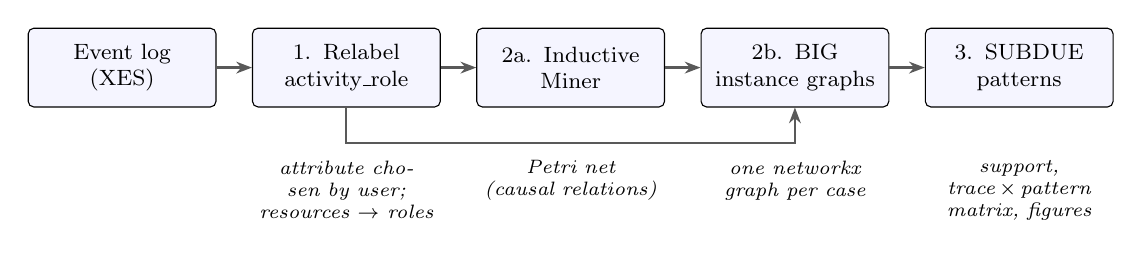
\begin{tikzpicture}[
  box/.style={draw, rounded corners=2pt, align=center, font=\footnotesize,
              minimum height=1cm, text width=2.15cm, fill=blue!4},
  data/.style={font=\scriptsize\itshape, align=center, text width=2.3cm},
  arr/.style={-{Stealth[length=2mm]}, thick, gray!70!black}]
\node[box] (log) {Event log\\(XES)};
\node[box, right=0.45cm of log] (pre) {1. Relabel\\activity\_role};
\node[box, right=0.45cm of pre] (net) {2a. Inductive\\Miner};
\node[box, right=0.45cm of net] (big) {2b. BIG\\instance graphs};
\node[box, right=0.45cm of big] (sub) {3. SUBDUE\\patterns};
\draw[arr] (log) -- (pre);
\draw[arr] (pre) -- (net);
\draw[arr] (net) -- (big);
\draw[arr] (big) -- (sub);
\draw[arr] (pre.south) |- ++(0,-0.45) -| (big.south);
\node[data, below=0.55cm of pre] {attribute chosen by user; resources $\to$ roles};
\node[data, below=0.55cm of net] {Petri net\\(causal relations)};
\node[data, below=0.55cm of big] {one networkx graph per case};
\node[data, below=0.55cm of sub] {support, trace\,$\times$\,pattern matrix, figures};
\end{tikzpicture}
\caption{Pipeline of the approach.}
\label{fig:pipeline}
\end{figure}

\paragraph{Input.} An event log (XES) with a case id, an activity and a
timestamp per event, plus at least one organizational attribute (e.g.\\
\texttt{org:resource}). The control flow is needed for the instance graphs, the
attribute for the organizational view.

\paragraph{Step 1: relabelling and roles.} The tool lists all attributes with
their level (event/trace), number of values, coverage and examples, and asks on
the command line which attribute to use. Every event is relabelled
\texttt{activity\_value}, an \emph{entity specification} in the terms
of~\cite{diamantini2016behavioral}; missing values become \texttt{UNKNOWN}.
Individual resources are often too fine: on BPI~2017 they give 3,338 labels,
half of which occur fewer than 10 times, and a first attempt with the 80\% most
frequent resources gave uninterpretable results. Resources are therefore
grouped into roles with the method of Burattin et al.~\cite{burattin2013roles}:
every activity starts as a role described by the multiset of its resources, and
the two most similar roles are merged while their similarity exceeds $\theta$
(default 0.65). Each resource gets its \emph{dominant role} (the one with most
of its events); labelling events with the role of their \emph{activity} would
add no information. Parameter $k$ keeps only the $k$ largest roles and merges
the rest into \texttt{Other}.

\paragraph{Step 2: instance graphs.} An instance graph~\cite{vandongen2004instance}
is a DAG of the events of one case whose edges are causal relations, so events
that may happen in any order lie on parallel branches. The relations come from
a Petri net discovered with the infrequent Inductive Miner (noise threshold
0.2, as in~\cite{diamantini2016behavioral}). BIG~\cite{diamantini2016big} aligns
every trace with the net, builds its instance graph and repairs inserted and
deleted events. Its text output is converted to one \texttt{networkx} graph per
case; every node gets a unique global id (the local id is kept) and its
activity and role, and graph $i$ is linked to case $i$.

\paragraph{Step 3: patterns.} All instance graphs form one disconnected graph
for SUBDUE~\cite{cook1994subdue,jonyer2002subdue}, matched on node labels with
directed edges. SUBDUE's beam search returns the subgraphs $s$ that best
compress the graph, value $=(k_s-1)|E_s|/|E|$ for $k_s$ non-overlapping
instances, preferring frequent and large patterns. With several
\emph{iterations}, the best pattern is compressed into one node and the search
is repeated, giving a pattern hierarchy~\cite{diamantini2016behavioral}.
Parameters: beam width (4 in~\cite{diamantini2016behavioral}), pattern size
(2--10 edges), patterns per iteration (3) and iterations. The output per
pattern is its graph, roles, number of instances (occurrence-based support),
number of cases containing it (transaction-based support) and a trace $\times$
pattern matrix; functions draw graphs, patterns, support and role handovers.

\section{Implementation}\label{sec:implementation}
Python~3.9 with pm4py~2.2.16 (as BIG requires), \texttt{networkx}, the provided
BIG and the Python SUBDUE (both unmodified); one module per step, a single
entry point with command-line parameters, and 40 unit tests. Three details
matter for reproducibility and run time. (i) pm4py's Inductive Miner iterates
over Python sets, so the hash seed is fixed; repeated runs then give identical
graphs. (ii) BIG handles $\approx$15 cases per minute; it runs on consecutive
chunks of the log in parallel and the outputs are joined in order (identical to
one run; 49 instead of $\approx$210 minutes on BPI). (iii) SUBDUE compares
candidates pairwise. We replace three of its helper functions at run time by
versions that first group candidates by a fingerprint that every matching pair
shares, keeping SUBDUE's own matcher and order: the output is identical
(tested), and 1,000 BPI graphs take 63\,s instead of 282\,s. SUBDUE's networkx
interface silently drops edge directions, so its input is built directly, and
its \emph{limit} is set so that every one-edge pattern is extended, since a
lower limit makes the result depend on the edge order.

\section{Evaluation Design and Results}\label{sec:evaluation}

\paragraph{Data.} (1) \emph{Synthetic logs} with a known ground truth: a
simplified loan process with four departments (Intake, Offer, Validation,
Decision; 16 employees) and 500 cases. Five work practices are injected
(Table~\ref{tab:synthetic}), two handovers and one with parallel work
(documents and fraud are checked in any order). Noise is added at four levels:
in 0, 10, 20 or 30\% of the cases one disturbance (event by an employee of
another department, extra event, missing event, or two events swapped). (2) The
\emph{BPI 2017} log of denied applications~\cite{vandongen2017bpi} (3,093 cases,
124,866 events, 54 activities, 134 resources), relabelled with
\texttt{org:resource}.

\paragraph{Design.} On the synthetic logs the whole pipeline runs, discovered
roles are mapped to departments via the employees, and the injected patterns
are the gold standard. A gold pattern is \emph{found} if a discovered pattern
contains it as a labelled subgraph; a discovered pattern is \emph{correct} if it
contains a gold pattern or is part of one; this gives precision, recall and F1.
As a baseline we use the most frequent label paths of 3 edges, as many as
SUBDUE returns (sequential pattern mining without compression). A parameter
study varies $k$, beam width and iterations. On BPI, where no ground truth
exists, we validate one instance graph against its trace, inspect the roles and
patterns, and compare with 9 expected work practices derived from the log
description and the role table (in the repository).

\begin{table}[t]
\centering\small
\caption{Injected work practices (synthetic log) and their recovery at 0\% / $\geq$10\% noise.}
\label{tab:synthetic}
\begin{tabular}{llcc}
\toprule
ID & Work practice & 0\% & $\geq$10\% \\
\midrule
G1 & Intake registers and checks & \checkmark & \checkmark \\
G2 & Handover Intake $\to$ Offer: call customer, complete application & \checkmark & \checkmark \\
G3 & Offer team creates and sends the offer & \checkmark & \checkmark \\
G4 & Validation checks documents $\parallel$ fraud, then decision & \checkmark & -- \\
G5 & Handover Decision $\to$ Offer: deny, notify customer & \checkmark & \checkmark \\
\bottomrule
\end{tabular}
\end{table}

\paragraph{Synthetic results.} Role discovery recovers the four departments
perfectly at every noise level (all employees in the right role). Without
noise, 71\% of the instance graphs contain the parallel branch and SUBDUE (5
iterations) finds all five practices with precision 0.93 (F1 0.97), clearly
above the baseline (F1 0.77), which cannot represent parallelism
(Figure~\ref{fig:synthetic}, Table~\ref{tab:results}). With 10\% noise or more, however, the Inductive
Miner no longer finds the parallel block, at any noise threshold from 0 to 0.8:
the noisy labels (24 instead of 12) change the discovered structure. All
instance graphs become sequences, G4 is lost and SUBDUE (F1 0.69) is no better
than the baseline (0.80). The parameter study on the 10\% log shows that the
number of iterations matters most: 3 iterations give F1 0.89 (precision 1.0),
1 iteration finds only 3 practices (F1 0.75), and 5--10 iterations add
fragments (precision 0.60--0.33). Beam width (2, 4, 10) has no effect on these
small graphs and only costs time; $k=2$ merges two departments into
\texttt{Other} without changing the scores.


\begin{table}[t]
\centering\small
\caption{Precision (P), recall (R) and F1 of the discovered patterns. Baseline: most
frequent label paths of 3 edges, same number of patterns.}
\label{tab:results}
\begin{tabular}{llrrrr}
\toprule
Log & SUBDUE configuration & P & R & F1 & Baseline F1 \\
\midrule
Synthetic, 0\% noise & 5 iterations, beam 4 & 0.93 & 1.00 & 0.97 & 0.77 \\
Synthetic, 10--30\% noise & 5 iterations, beam 4 & 0.60 & 0.80 & 0.69 & 0.80 \\
Synthetic, 10\% noise & 1 iteration (any beam, $k$) & 1.00 & 0.60 & 0.75 & -- \\
Synthetic, 10\% noise & 3 iterations (any beam, $k$) & 1.00 & 0.80 & 0.89 & -- \\
Synthetic, 10\% noise & 10 iterations (any beam, $k$) & 0.33 & 0.80 & 0.47 & -- \\
\midrule
BPI 2017 & 1 iteration, beam 4 & 1.00 & 0.33 & 0.50 & -- \\
BPI 2017 & 10 iterations, beam 4 & 0.63 & 0.89 & 0.74 & 0.72 \\
BPI 2017 & 10 iterations, beam 10 & 0.77 & 0.89 & 0.82 & 0.72 \\
BPI 2017 & 10 iterations, beam 20 & 0.87 & 1.00 & 0.93 & 0.72 \\
\bottomrule
\end{tabular}
\end{table}

\begin{figure}[t]
\centering
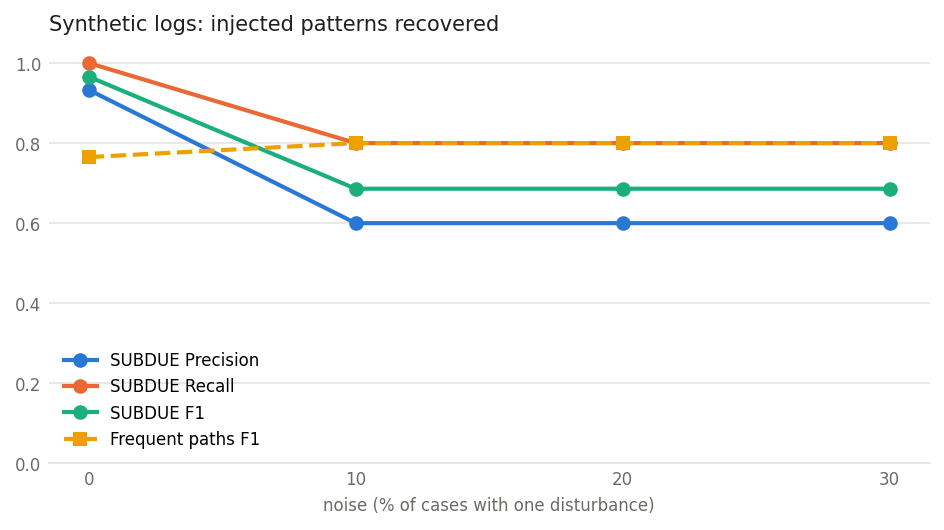
\includegraphics[width=0.62\textwidth]{figures/synthetic_results.png}
\caption{Synthetic logs: SUBDUE (5 iterations, beam 4) and frequent-path baseline per noise level.}
\label{fig:synthetic}
\end{figure}

\paragraph{BPI 2017 results.} Role discovery groups the 134 resources into 8
roles (3,338 $\to$ 225 labels): Role\_1 (86 users) completes applications and
handles offers, Role\_2 (21) validates, Role\_3 (18) handles fraud, incomplete
files and denials, Role\_4 (2, incl.\ the system user) registers applications;
roles 5--8 are small (3, 2, 1, 1 users). For case Application\_1691306052 the
instance graph (Figure~\ref{fig:ig}) matches the trace exactly: 33 events and nodes with the same
labels, the right role for every event, and all 32 edges between consecutive
events. As in the noisy synthetic logs, only 0.3\% of the 3,093 graphs contain
parallel branches: the net has one AND-split, also on plain activities, whereas
the net provided with the assignment has five. The hierarchical run finds a
different process phase in every iteration (Table~\ref{tab:patterns}), e.g.\ the offer team (Role\_1)
handing cases to the validation team (Role\_2) after calling the customer
(Figure~\ref{fig:pattern}, 61\% of the cases), and the intake (Role\_4) handing
over to Role\_1 (45\%). Over all graphs 80--93\% of the edges stay within a role
(Figure~\ref{fig:handover}). Against the 9 expected practices (Table~\ref{tab:results}), beam width does
matter on this large graph: F1 0.74 (beam 4), 0.82 (10) and 0.93 (20, all 9
found), above the baseline (0.72 for paths of 3 edges, 0.80 for 4 edges), at
10, 13 and 16 minutes. A single iteration
finds only 3 of 9 (F1 0.50) because its patterns are variants of one sequence.
Failed cases: incomplete-file handling is split between two roles (37/55\%),
which fragments its labels; and \texttt{A-Concept} is shared 46/53\% by Role\_1
and Role\_4, so patterns with either role count as only half right.


\begin{figure}[t]
\centering
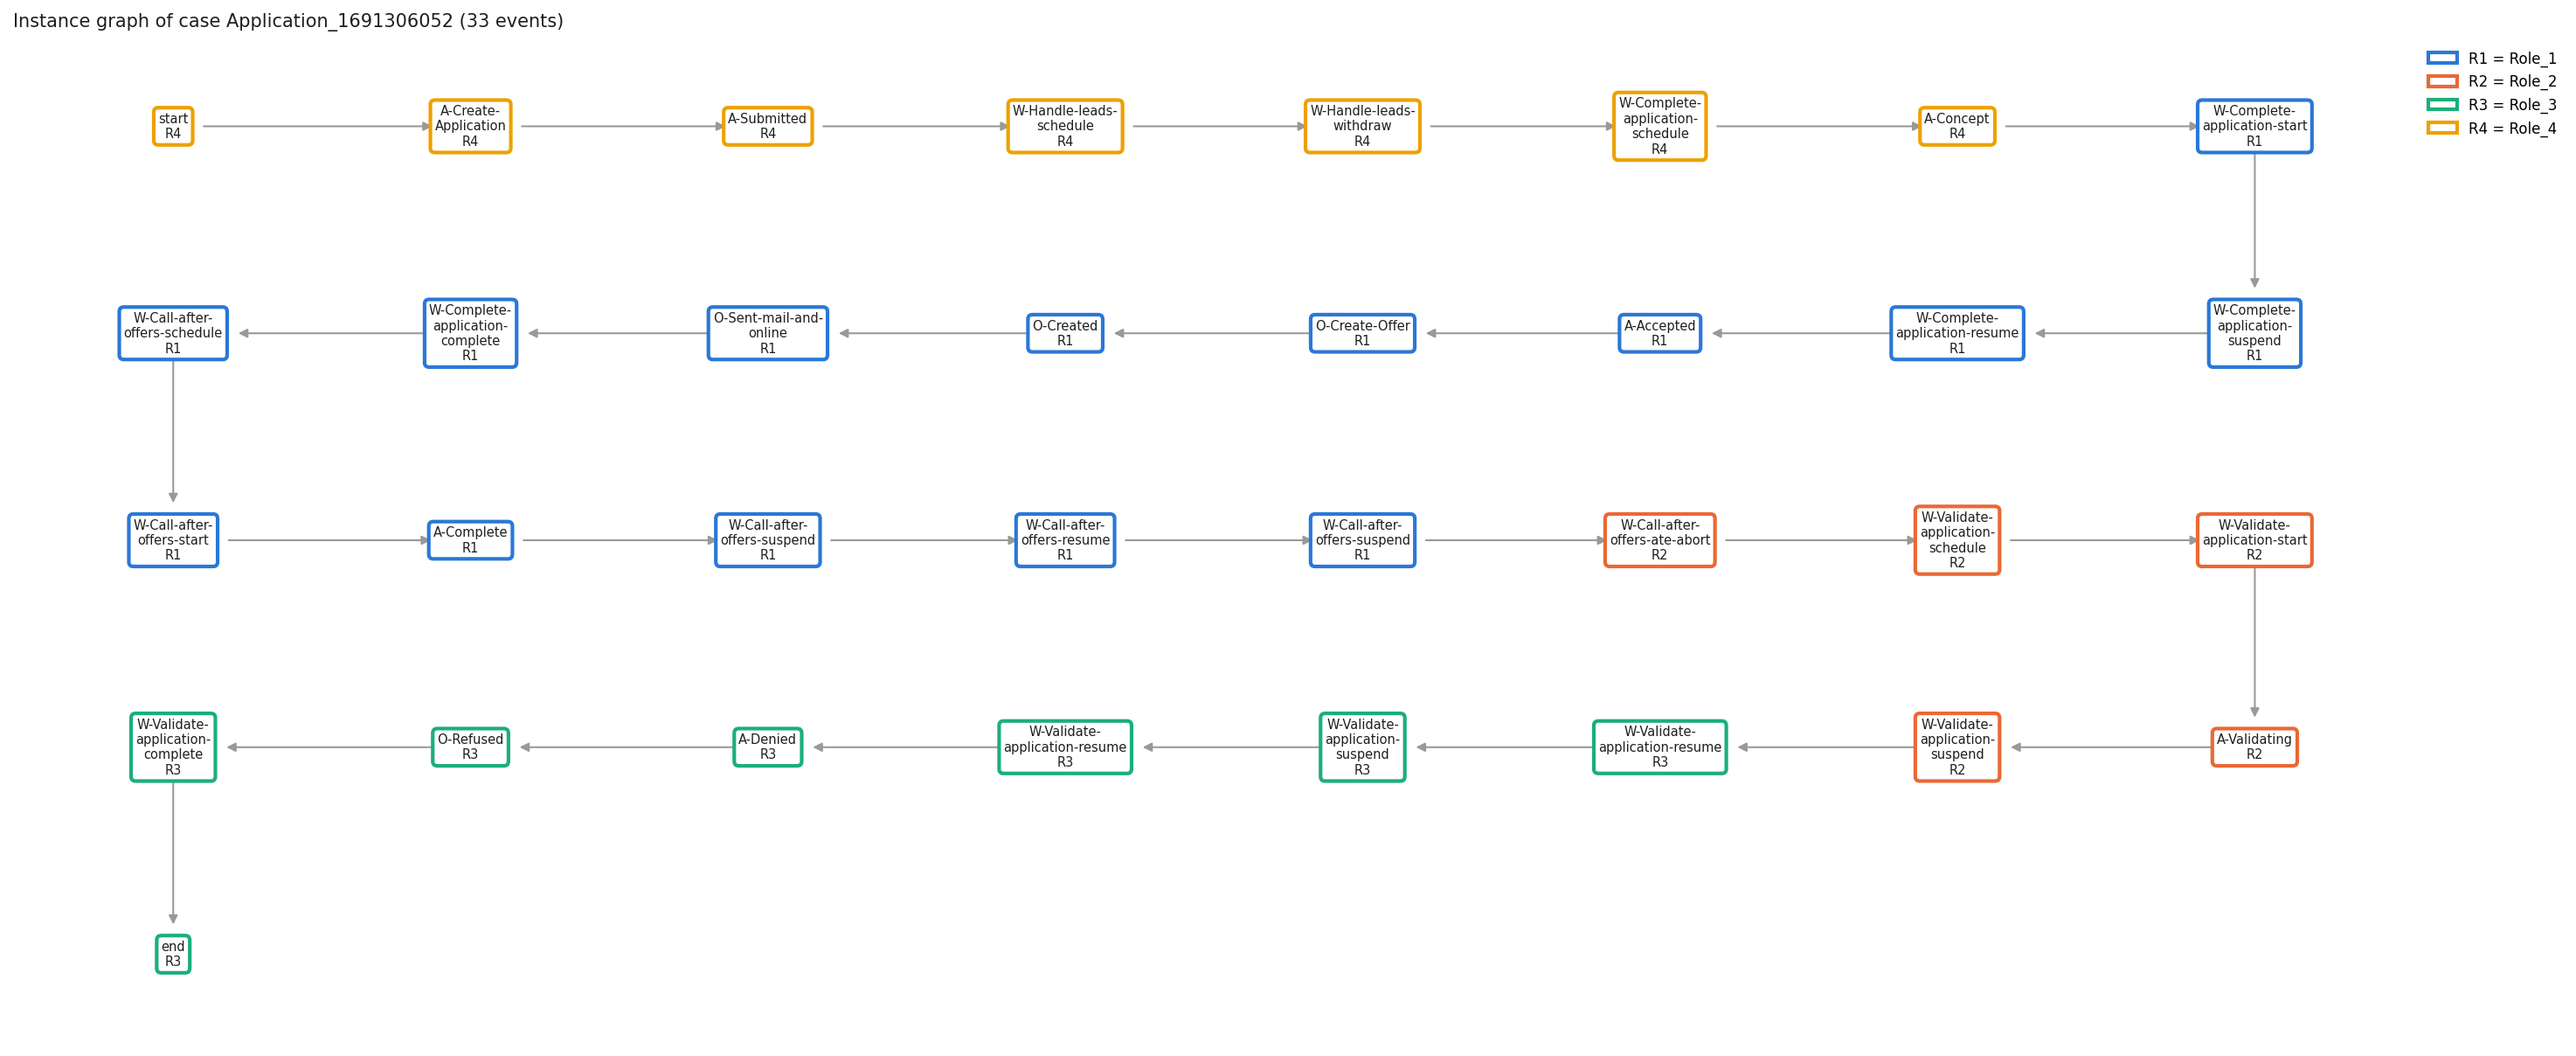
\includegraphics[width=\textwidth]{figures/instance_graph_example.png}
\caption{Instance graph of BPI case Application\_1691306052 (read as a snake: left to
right, then right to left). The case passes from the intake (R4) to the offer team
(R1), validation (R2) and decision (R3); every edge links two consecutive events.}
\label{fig:ig}
\end{figure}

\begin{table}[t]
\centering\small
\caption{BPI 2017: best pattern of the first iterations (10 iterations, beam 4).}
\label{tab:patterns}
\begin{tabular}{llrlr}
\toprule
Pattern & What it shows & Edges & Roles & Cases \\
\midrule
P1.1 & Offer team calls after the offer, validation takes over & 10 & R1, R2 & 61\% \\
P2.1 & Intake registers the application, R1 continues & 7 & R4, R1 & 45\% \\
P3.1 & Application accepted, offer created and sent & 3 & R1 & 82\% \\
P4.1 & Call for incomplete files, validation takes over & 6 & R1, R2 & 23\% \\
P7.1 & Denied, offer refused, case ends & 3 & R3 & 31\% \\
\bottomrule
\end{tabular}
\end{table}

\begin{figure}[t]
\centering
\begin{subfigure}[b]{0.6\textwidth}
  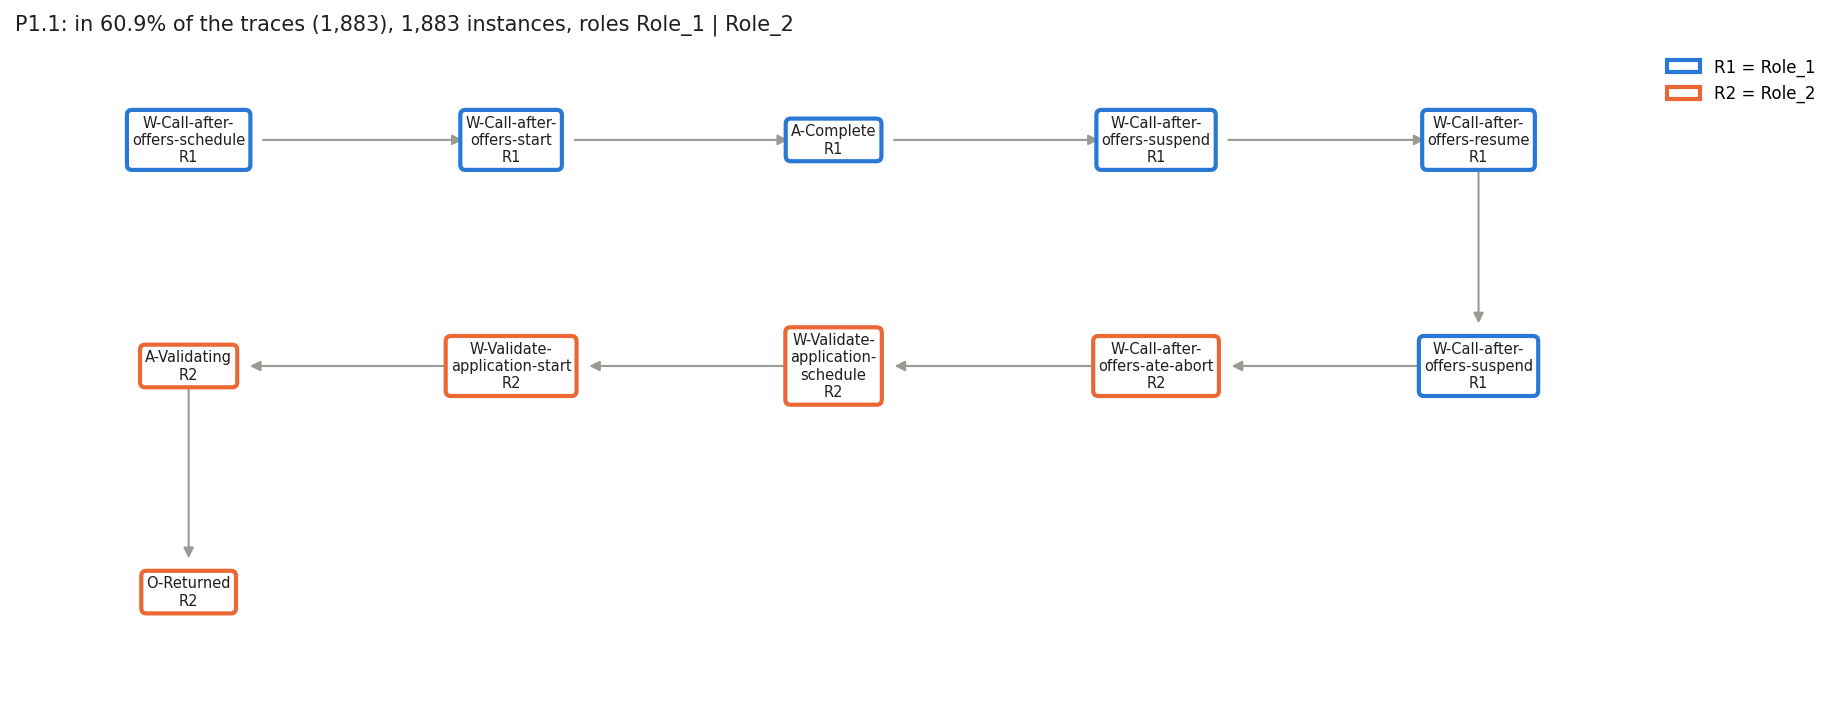
\includegraphics[width=\textwidth]{figures/pattern_P1_1.png}
  \caption{Pattern P1.1: offer team (R1) $\to$ validation team (R2).}
  \label{fig:pattern}
\end{subfigure}\hfill
\begin{subfigure}[b]{0.38\textwidth}
  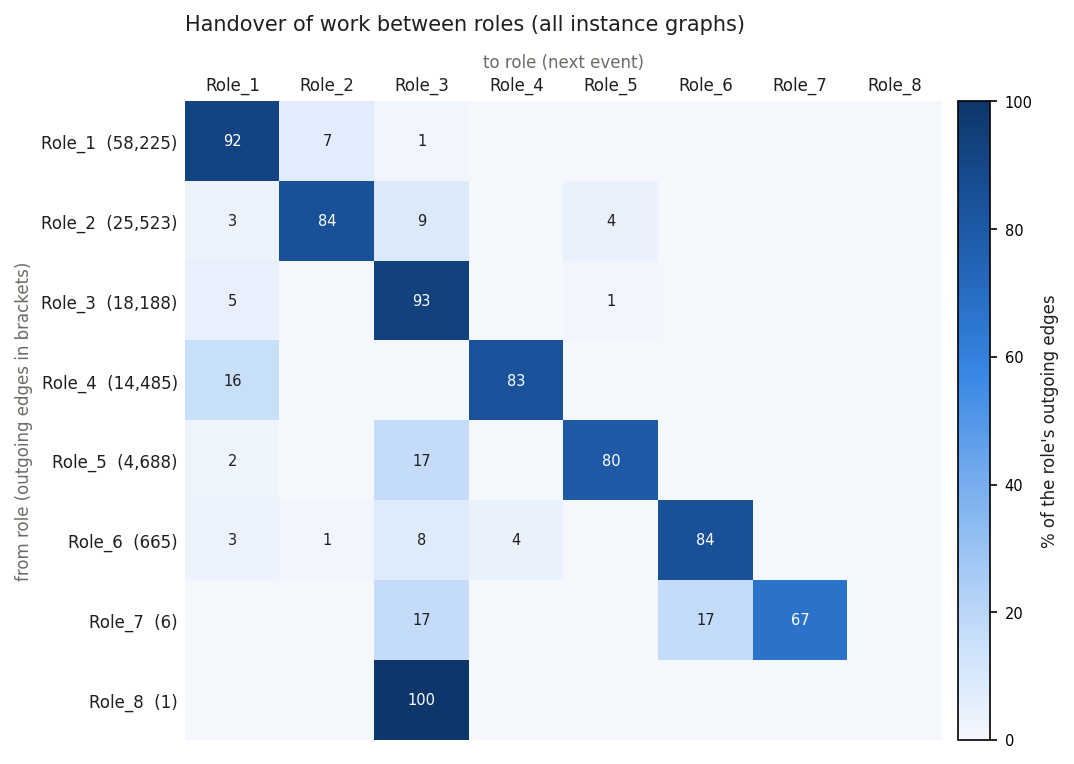
\includegraphics[width=\textwidth]{figures/role_handover.png}
  \caption{Handover of work between roles.}
  \label{fig:handover}
\end{subfigure}
\caption{BPI 2017: a discovered handover pattern and the handovers over all instance graphs.}
\end{figure}

\section{Limitations and Future Work}\label{sec:limitations_futurework}
\textbf{Process model.} The synthetic logs show the main limitation: pm4py's
Inductive Miner loses parallelism under modest noise, after which instance
graphs are sequences and graph mining has no advantage over sequential
patterns. This explains the BPI results. Future work: other miners, or causal
relations derived from the activity-level model and lifted to the role labels.
\textbf{Roles.} Dominant-role assignment yields tiny roles on BPI (top-$k$
helps) and one large role (86 users); activities shared by roles fragment
patterns. Assigning roles per event, or a higher $\theta$, should be tested.
\textbf{Evaluation.} The synthetic process is small and its noise model simple;
the BPI reference practices were written by us after seeing first results.
Larger synthetic processes with known roles, and the structural measures of
\cite{diamantini2016behavioral} (coverage, diversity), are next steps.
\textbf{Search.} Later iterations add fragments; the number of iterations
should be chosen per log, e.g.\ by stopping when patterns become small.

\printbibliography

\section{Technology Statement}
During the preparation of this work, I/We used [NAME TOOL / SERVICE / VERSION OF AI
TOOL] in order to [REASON]. The following parts of the assignment were
affected/generated by AI tool usage: [INTRODUCTION / METHODS / xxx, DISCUSSION].
After using this tool/service, [NAME STUDENT(S)] evaluated the validity of the tool's
outputs, including the sources that generative AI tools have used, and edited the
content as needed. As a consequence, [NAME STUDENT (S)] take(s) full responsibility
for the content of their work

\end{document}
